\section{Experimental setup}
\label{sec:setup}
The minimum-bias (MB) events in p--Pb collisions at $\snn$~=~5.02~TeV used for the present analysis are recorded by the ALICE detector in 2016. The nucleon–nucleon centre-of-mass system is shifted by $\Delta \mathrm{y}_{\mathrm{cms}} =$~0.465 in the unit of rapidity along the direction of the proton beam. The entire subsystem of the ALICE detector can be found in Ref.~\cite{Abelev:2014ffa} for the LHC Run 2 period. The present analysis is carried out with the Inner Tracking System (ITS)~\cite{ALICE:2010tia}, the Time Projection Chamber (TPC)~\cite{Alme:2010ke}, the Time-Of-Flight (TOF)~\cite{Jacazio:2018slq}, V0~\cite{ALICE:2013axi}, and the Zero Degree Calorimeter (ZDC)~\cite{Cortese:2019nnv}. 

The V0 detector has two stations located at both forward sides with respect to the nominal interaction point, V0A and V0C, each made of 32 plastic scintillator strips, covering the full azimuthal angle within the pseudorapidity intervals $2.8 < \eta < 5.1$ and $-3.7 < \eta < -1.7$, respectively. V0A detector on Pb-going side is used to provide a MB trigger in p--Pb collisions. The V0A provides the multiplicity class using the sum of the V0A signals at the same time. The collected data samples from the MB trigger correspond to the integrated luminosity of 0.24~nb$^{-1}$~\cite{ALICE:2014gvw}. The ZDC which detects ``slow'' nucleons at very large $\eta$~\cite{Cortese:2019nnv} also defines the most unbiased multiplicity class. The multiplicity of neutrons by nuclear de-excitation processes or neutrons knocked out from wounded nucleons is expected to increase with the number of nucleon–nucleon binary collisions at the Pb-going side~\cite{ALICE:2014xsp}. This multiplicity definition is the least-biased centrality estimator for p--Pb collisions.

%The V0A detector is utilized to measure the particle yield ratio of \fzero~because the multiplicity dependence of $\mathrm{K}^{*0}$ and $\pi$ yields are measured with the V0A detector. The ZDC which detects ``slow'' nucleons at very large $\eta$~\cite{Cortese:2019nnv}  also defines the most unbiased multiplicity class for the event selection. The multiplicity dependence of the nuclear modification factor of \fzero~is measured using the hybrid method, which can be conducted with the ZDC~\cite{ALICE:2014xsp}, to scale down the cross section of the \fzero~in p--Pb collisions with a reduced bias.

The primary vertex position is reconstructed using the measured track segments in the Silicon Pixel Detector (SPD)~\cite{Santoro2009:ALICESPD}, which is the innermost two layers of the ITS. The reconstructed primary vertex is required to be within 10~cm from the center of the detector along the beam direction. Pileup events are rejected when multiple primary vertices are reconstructed and the longitudinal displacement of their reconstructed vertices is larger than 0.8~cm. The probability of pileup events is expected to be 0.5\% in MB events. The TPC is the main tracking detector of ALICE, covering a pseudorapidity range $|\eta|<$~0.9 over the full azimuth in a uniform solenoidal magnetic field of 0.5~T along the beam axis. The TPC can reconstruct charged tracks originating from the primary vertex down to $p_{\rm{T}}=$~0.1~GeV/$c$. Particle identification (PID) can be done with the TPC and TOF. The TPC measures ionization energy loss $\mathrm{d}E/\mathrm{d}x$ of charged tracks to separate particle species. The TOF helps the PID capabilities of the TPC by measuring the flight time of charged particles from the interaction point to the TOF.

\section{Data analysis}
\label{sec:ana}
\begin{figure}[hbt!]
	\centering
	\subfigure{ 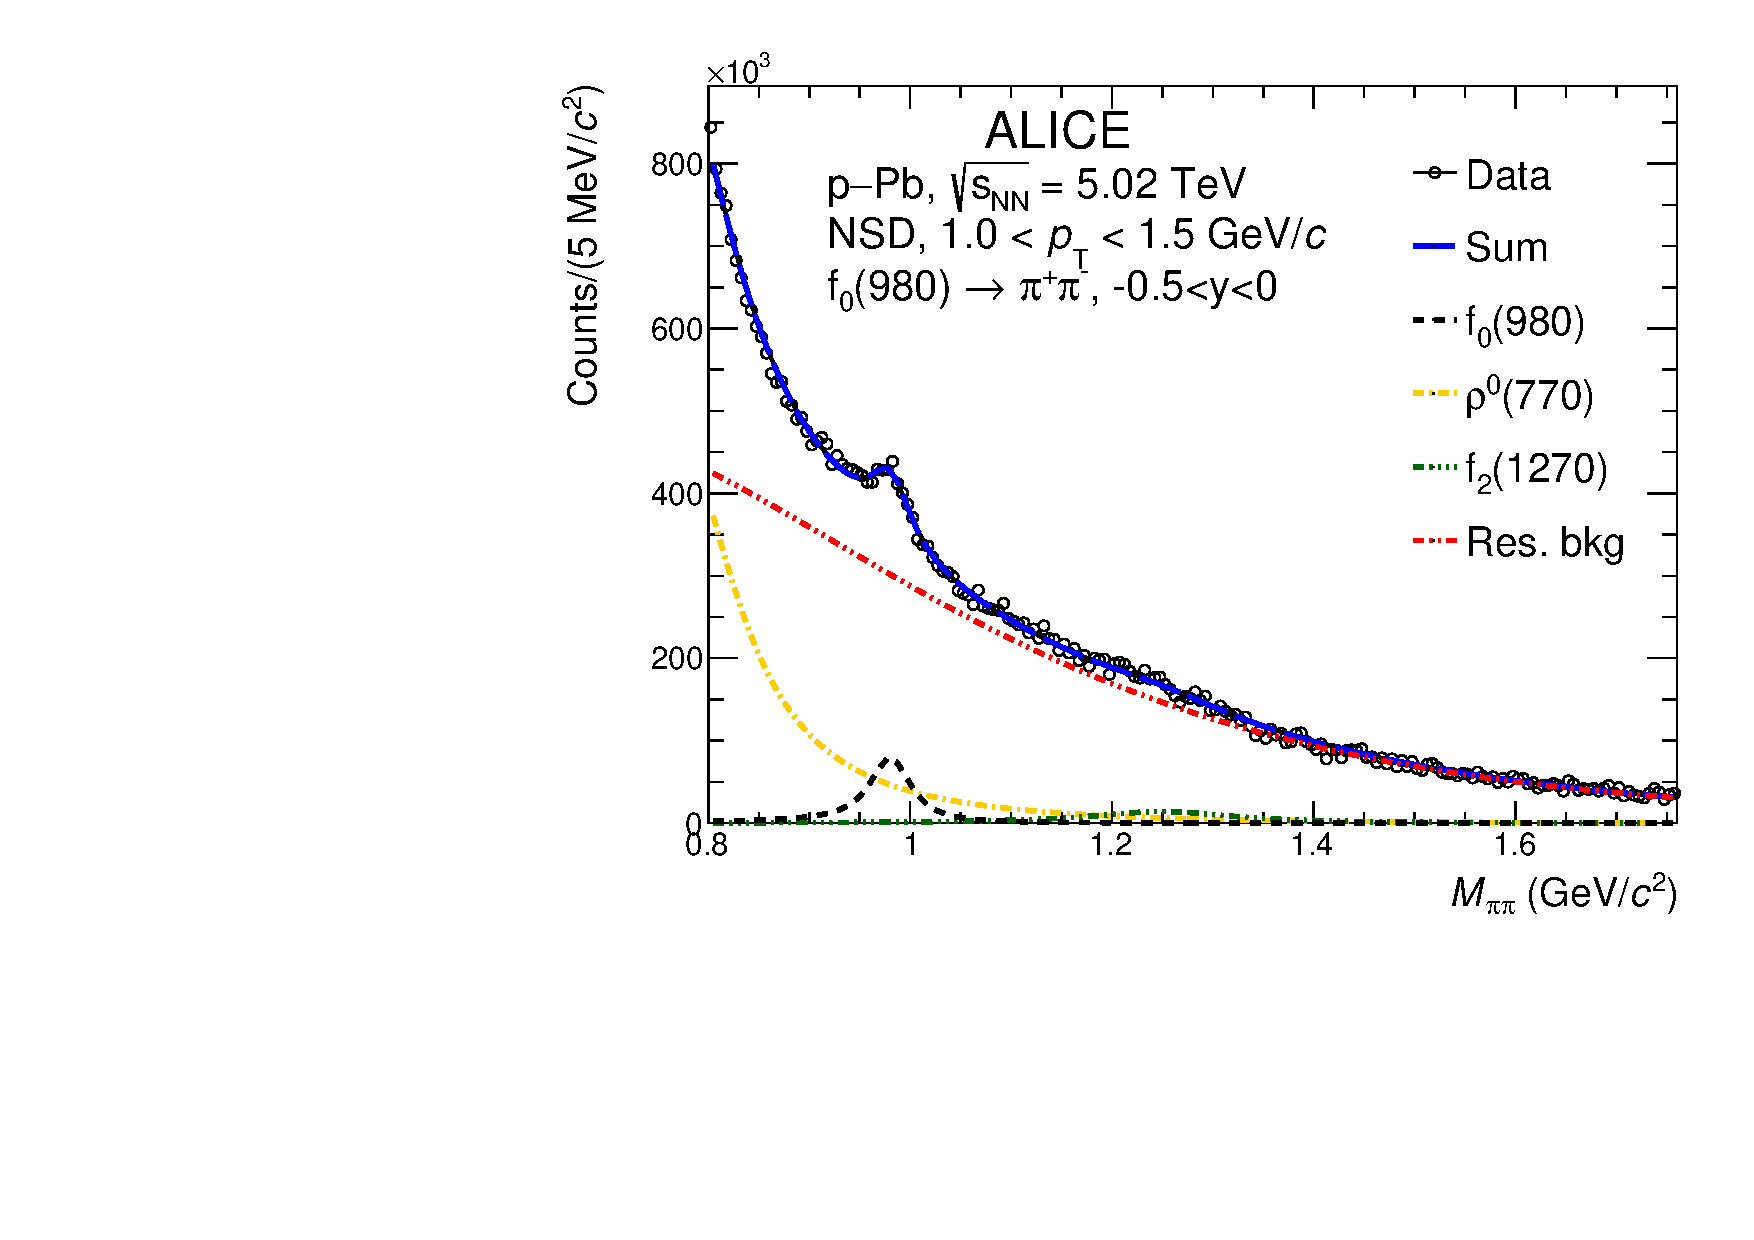
\includegraphics[width=0.47 \textwidth]{figures/Fig1_sigext_mb_0pt_mb.pdf} }
	\subfigure{ 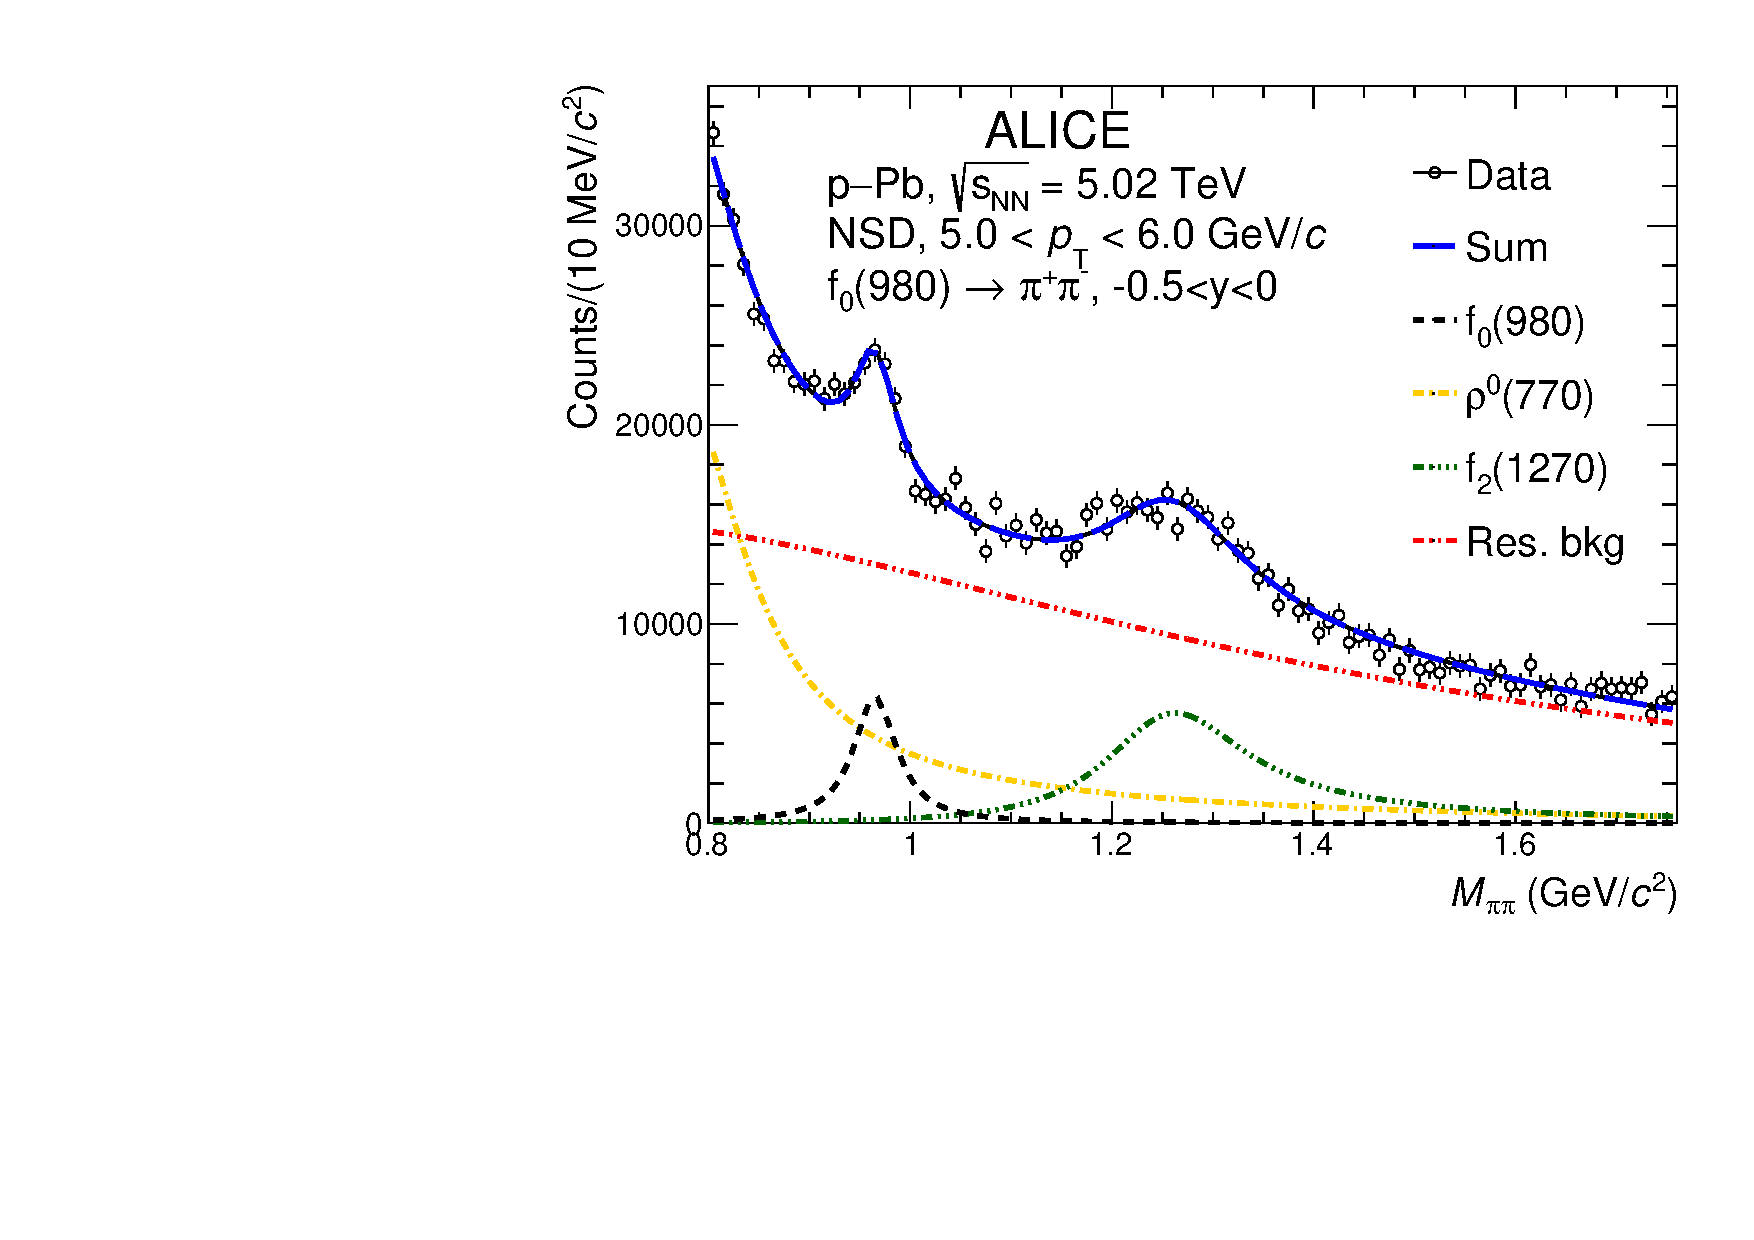
\includegraphics[width=0.47 \textwidth]{figures/Fig1_sigext_mb_1pt_mb.pdf} }
	\caption{ Invariant mass distribution of $\pi^{+}\pi^{-}$ pairs in -0.5~$<\mathrm{y}<$~0 after like-sign backgrounds subtraction in p--Pb collisions at \snn~=~5.02~TeV. The left (right) plot is obtained at low (high) $p_{\mathrm{T}}$ of $\pi^{+}\pi^{-}$ pairs in non-single diffraction (NSD) events }
	\label{fig:SigExt}
\end{figure}

The \fzero~is reconstructed with the decay channel of \fzero~$\rightarrow \pi^{+}\pi^{-}$, where the branching ratio of the decay is 46~$\pm$~6\%~\cite{Stone:2013eaa}. Each charged pion is required to have $p_{\rm{T}}>$~0.15~GeV/$c$ and $|\eta|<$~0.8 for a uniform detector acceptance. The reconstructed tracks are required to satisfy selection criteria listed in the previous work~\cite{ALICE:2018qdv} to guarantee the good reconstruction of charged tracks. In particular, the number of horizontal segments for the transverse readout is required to be in 70--159 for the TPC track. A $p_{\mathrm{T}}$-dependent selection criteria on the distance of closest approach to the primary vertex in the transverse ($d_{z}$) and the longitudinal ($d_{xy}$) direction is required to be $d_{z}<$~2~cm and $d_{xy}<$~(0.0105~$+$~0.0350~$\times p_{\mathrm{T}}^{-1.1})$~cm, respectively, to suppress contaminations from secondary charged particles originating from weakly decaying hadrons.

The identification of charged pions is done with the combined information of the TPC and TOF. The difference of the ionization energy loss between the prediction from Bethe-Block parametrization with the pion mass assumption and measured energy is required to be within two standard deviations to identify pions for the TPC. The difference of flight time between the prediction with the pion mass assumption and measured time is required to be within three standard deviations to identify pions for the TOF. The TOF is not used for the particle identification when the TOF track is not identifiable.

The pair of two charged pions is selected in -0.5~$<\mathrm{y}<$~0, where $\mathrm{y} = -\mathrm{y}_{\mathrm{lab}} -0.465$~\cite{ALICE:2017pgw}. The combinatorial backgrounds are subtracted using the like-sign method~\cite{PhysRevD.36.2019}. The like-sign backgrounds are constructed as the geometric average of $\pi^{+}\pi^{+}$ and $\pi^{-}\pi^{-}$ distributions,  2$\sqrt{N^{\pi^{+}\pi^{+}}N^{\pi^{-}\pi^{-}}}$. After subtracting the like-sign backgrounds from $\pi^{+}\pi^{-}$ distribution, peaks of resonances decaying to $\pi^{+}\pi^{-}$ can be identified. Figure~\ref{fig:SigExt} shows the like-sign-subtracted $\pi^{+}\pi^{-}$ invariant mass distributions for 1.0~$<p_{\rm{T}}<$~1.5~GeV/$c$ (5.0~$<p_{\rm{T}}<$~6.0~GeV/$c$) in MB events on the left (right) plot. Because $\rho$(770) and $\rm{f}_{2}$(1270) dominantly decay to $\pi^{+}\pi^{-}$, \fzero~signals are overlapped with contributions from $\rho$(770) and $\rm{f}_{2}$(1270). Additional backgrounds are attributed to misidentified particles and mini-jets, which are represented as red-dashed-dotted lines in Fig.~\ref{fig:SigExt}. Each resonance contribution is described with relativistic Breit-Wigner function (rBW)~\cite{ALICE:2018qdv, ALICE:2022qnb} because detector resolution is expected to be negligible with respect to the width of the \fzero. The rBW can be expressed as
\begin{eqnarray}
\mathrm{rBM}(M_{\pi\pi}) = \dfrac{AM_{\pi\pi}\Gamma(M_{\pi\pi})M_{0}}{(M_{\pi\pi}^{2}-M_{0}^{2})^{2} + M_{0}^{2}\Gamma^{2}(M_{\pi\pi})},
\label{eq:rBW}
\end{eqnarray}
where $\Gamma(M_{\pi\pi})$ is denoted as
\begin{eqnarray}
\Gamma(M_{\pi\pi}) = \left[ \dfrac{ (M_{\pi\pi}^{2} - 4m_{\pi}^{2}) }{ (M_{0}^{2}-4m_{\pi}^{2}) } \right]^{(2J+1)/2} \times \dfrac{\Gamma_{0}M_{0}}{M_{\pi\pi}}
\label{eq:rBWW}
\end{eqnarray}
$A$ and $M_{0}$ in Eq~\ref{eq:rBW} are the amplitude of the rBW and the rest mass of the resonance, respectively. $\Gamma_{0}$, $J$, and $m_{\pi}$ are the rest width of the resonance, the spin, and the charged pion mass, respectively. The spins for \fzero~, $\rho$(770), and $\mathrm{f}_{2}$(1270) are 0, 1, and 2, respectively. Residual backgrounds ($f_{\mathrm{bkg}}$) is expressed with a Maxwell-Boltzmann-like distribution, which can be expressed as~\cite{OPAL:1998enc}
\begin{eqnarray}
f_{\mathrm{bkg}}(M_{\pi\pi}) = B(M_{\pi\pi}-2m_{\pi})^{n}\exp{(c_{1}M_{\pi\pi} + c_{2}M_{\pi\pi}^{2})}.
\label{eq:bkg}
\end{eqnarray} 
Each rBW of the resonance is corrected for the invariant mass dependent $\pi\pi$ interference~\cite{Rapp:2003ar}, which can be expressed as
\begin{eqnarray}
\mathrm{PS}(M_{\pi\pi}) = \dfrac{M_{\pi\pi}}{\sqrt{M_{\pi\pi}^{2}+p_{\mathrm{T}}^{2}}}\times\exp{(-\sqrt{M_{\pi\pi}^{2}+p_{\mathrm{T}}^{2}}/T_{\mathrm{kin}})},
\label{eq:ps}
\end{eqnarray} 
where $p_{\mathrm{T}}$ in the above equation denotes the transverse momentum of the $\pi\pi$. $T_{\mathrm{kin}}$ is the kinetic freeze-out temperature and set to be 160~MeV~\cite{ALICE:2013wgn} for different multiplicity classes.

The signal extraction carefully considers the width of the \fzero~as the width is not well known yet (10~$<\Gamma_{0}^{\mathrm{f}_{0}}<$~100~MeV/$c^{2}$~\cite{ParticleDataGroup:2020ssz}). The total fit function consists of three rBWs and $f_{\mathrm{bkg}}$. Total fit function consists of three rBWs and $f_{\mathrm{bkg}}$, which is constructed with 9 fit parameters as the masses and widths of $\rho$(770) and $\mathrm{f}_{2}$(1270) are well defined in Ref.~\cite{ParticleDataGroup:2020ssz}, and those are fixed to $m{\rho}=$~775.3~MeV/$c^{2}$, $\Gamma_{\rho}=$~~149.1~MeV/$c^{2}$, $m_{\mathrm{f}_{2}}=$~1,275.5~MeV/$c^{2}$, and $\Gamma_{\mathrm{f}_{2}}=$~186.7~MeV/$c^{2}$ during all fit procedures. Due to the many free parameters during the fit, the procedure is split into three steps to prevent fit results from being in local minima and to minimize possible biases to the estimation on the rBW for \fzero. The purpose of the first step is to obtain unbiased \fzero~width, which is called initial \fzero~width. To accumulate enough statistics, the first step is only conducted in MB events for merged $p_{\mathrm{T}}$ ranges. During the first step, all parameters are left free. The second step is conducted to constrain the $f_{\mathrm{bkg}}$. In the second step, the \fzero~width is fixed as the initial \fzero~width, which is determined in the first step. The last fit procedure is processed with the fixed $f_{\mathrm{bkg}}$, while the \fzero~width is set free inside (10~$<\Gamma_{0}^{\mathrm{f}_{0}}<$~100~MeV/$c^{2}$. In each step, the fit range is set to 0.8~$<M_{\pi\pi}<$~1.76~GeV/$c^{2}$.

The previous analysis for the \fzero~production in pp collisions at $\sqrt{s}=$~5.02~TeV~\cite{ALICE:2022qnb} constrains the \fzero~width to be 55~MeV/$c^{2}$, while the present analysis sets the \fzero~width free. In the previous analysis, there is no phase space correction, which is expressed in Eq~\ref{eq:ps}. The present analysis considers the phase space correction for possibly larger $\pi\pi$ interference. It is found that consistent results are obtained from different analysis methods.

The raw \fzero~yields from the fit procedure are corrected for the acceptance and the tracking efficiency, and normalized for the event selections and the branching ratio~\cite{ALICE:2022qnb}, which can be expressed as
\begin{eqnarray}
\dfrac{1}{N_{\mathrm{NSD}}}\dfrac{\mathrm{d}^{2}N}{\mathrm{dyd}p_{\mathrm{T}}} = \dfrac{1}{N_{\mathrm{evt}}} \dfrac{ N_{\mathrm{f}_{0}} }{ \Delta \mathrm{y} \Delta p_{\mathrm{T}} } \dfrac{  \epsilon_{\mathrm{trig}} f_{\mathrm{vtx}} f_{\mathrm{S.L.}} }{\mathrm{Acc} \times \epsilon \times \mathrm{B.R.} }.
\end{eqnarray}
Here, $N_{\mathrm{evt}}$ is the number of events satisfying event selection criteria in the specific multiplicity class. $N_{\mathrm{f}_{0}}$ is the integration for the \fzero~rBW. $\Delta \mathrm{y}$ ($\Delta p_{\mathrm{T}}$) is the rapidity (transverse momentum) interval where the measurement is conducted. Coefficients for the acceptance and the tracking efficiency ($\mathrm{Acc}\times\epsilon$) are estimated from a detailed simulation for the ALICE detector responses. The p--Pb events are simulated using the DPMJET~\cite{Fedynitch:2015kcn} event generator with the artificial injection of \fzero~signals. Signals and backgrounds are transported through the detector using GEANT3~\cite{Brun:1994aa}. $\mathrm{Acc}\times\epsilon$ is estimated to be 26\% and gradually increasing up to 60\% as $p_{\mathrm{T}}$ increases and not dependent on the multiplicity class. $\mathrm{B.R.}$ is the branching ratio of the \fzero~$\rightarrow \pi^{+}\pi^{-}$ decay channel. The \fzero~yield is normalized for the trigger efficiency ($\epsilon_{\mathrm{trig}}$), vertex reconstruction efficiency ($f_{\mathrm{vtx}}$), and signal loss ($f_{\mathrm{S.L.}}$) due to the event selection. $\epsilon_{\mathrm{trig}}$ is estimate to be dependent on the multiplicity class and to increase from 0.84 to 1 as the multiplicity increases. $f_{\mathrm{vtx}}$ is estimated to be larger than 0.99 in all measured multiplicity classes. Because current realistic  simulations rarely produce primary \fzero, $f_{\mathrm{S.L.}}$ is estimated using the different particle, $\phi$ meson with the universal $m_{\mathrm{T}}$ scaling~\cite{Altenkamper:2017qot}. The former analysis shows $f_{\mathrm{S.L.}}$ does not depend on particle spices~\cite{ALICE:2019xyr}. $f_{\mathrm{S.L.}}$ is 1.03 for 0~$<p_{\mathrm{T}}<$~0.3~GeV/$c$ and saturated with 1 for $p_{\mathrm{T}}>$~2~GeV/$c$.

 
The comparison of the $p_{\rm{T}}$-differential invariant yield between p--Pb and pp collisions, which is called the nuclear modification factor ($Q_{\mathrm{pPb}}$), can be expressed as
\begin{eqnarray}
Q_{\mathrm{pPb}} = \dfrac{\mathrm{d}^{2} N_{\mathrm{f}_{0}(980)}^{\mathrm{pPb}} / \mathrm{d} p_{\mathrm{T}} \mathrm{dy} }{ \left\langle T_{\mathrm{pPb}} \right\rangle \mathrm{d}^{2} \sigma_{\mathrm{f}_{0}(980)}^{\mathrm{pp}}/ \mathrm{d} p_{\mathrm{T}} \mathrm{dy} },
\end{eqnarray}
where $\left\langle T_{\mathrm{pPb}} \right\rangle$ and $\sigma_{\mathrm{f}_{0}(980)}^{\mathrm{pp}}$ are the average nuclear overlap from the Glauber model~\cite{Miller:2007ri} and the cross section of \fzero~in pp collisions~\cite{ALICE:2022qnb}, respectively.

\section{Systematic uncertainties}
\label{sec:syst}
The systematic uncertainties of invariant yields are estimated by varying the analysis selection criteria and corrections, which are summarized in Tab.~\ref{tab:syst}. Total systematic uncertainty is calculated as a quadrature of each uncertainty. 

\begin{table}[h!]
\caption{The relative systematic uncertainty of invariant $p_{\rm{T}}$-differential yields. Numbers given in ranges correspond to minimum and maximum uncertainties.}
\centering
\begin{tabular}{cc|c}
\hline 
\multicolumn{2}{c|}{Sources}  &Systematic uncertainty (\%) \\ \hline
\multicolumn{2}{c|}{Primary vertex} & negligible \\ 
\multicolumn{2}{c|}{Tracking} & $\pm$4--6 \\
\multicolumn{2}{c|}{Particle identification} & $\pm$4--12 \\ 
\multirow{4}{*}{Signal extraction} &  $\mathrm{f}_{2}$(1270) parameters	& $\pm$3--9 \\ 
& $\rho$(770) parameters & $\pm$3--8 \\
& Fit range & $\pm$0--6 \\
& Init. $\mathrm{f}_{0}$ width & $\pm$2--12 \\
\multicolumn{2}{c|}{Phase space correction} & $\pm$3--8 \\ \hline 
\multicolumn{2}{c|}{Total (in quadrature)}	& $\pm$15--27 \\ 
\hline 
\end{tabular}
\label{tab:syst}
\end{table}

The systematic uncertainty from the primary vertex selection is tested by narrowing the requirement to 7~cm and the uncertainty is estimated to be negligible. The systematic uncertainty from the pileup rejection is tested by varying the minimal number of track contributors required for reconstruction of pileup event vertices from 5 to 3 and the uncertainty is estimated to be negligible.

The systematic uncertainty from tracking is assigned as the value from~\cite{ALICE:2013wgn}, where uncertainties are evaluated by varying the requirements of $d_{xy}$, $d_{z}<$, and the number of fired TPC readout channels. The systematic uncertainty from the particle identification is tested with different requirements on the number of standard deviations by $\pm\,0.5\sigma$ for the TPC and the TOF, and the uncertainties are estimated to be 4--12\%.

The systematic uncertainties from masses and widths of $\mathrm{f}_{2}$(1270) and $\rho$(770) are evaluated by shifting the masses and the widths as much as three times their measured statistical uncertainties, which are reported at Ref~\cite{ParticleDataGroup:2020ssz}. The estimated uncertainties from $\mathrm{f}_{2}$(1270) and $\rho$(770) parameters are 3--9\% and 3--8\%, respectively. The systematic uncertainty from the fit range is estimated by changing the range inward or outward as much as 40~MeV/$c^{2}$. The uncertainties are estimated to be 0--6\%.

The systematic uncertainty from the initial \fzero~width, which is obtained in the first step describe in Sec.~\ref{sec:ana}, is estimated by varying the width as much as their measured statistical uncertainties in both directions. The changes affect the background distribution determined in the second step. The estimated systematic uncertainties are 2--12\%.

The systematic uncertainty from phase space correction is estimated by varying the kinetic freeze-out temperature in the range of 140~$<T_{\mathrm{kin}}<$~180~MeV. The estimated uncertainties are 3--8\%. 

The multiplicity dependent correlations of uncertainties are evaluated by quantifying how much uncertainties collectively varies in the same direction with respect to the multiplicity class. Total uncorrelated systematic uncertainties are about half of total systematic uncertainties for all inspected sources.







\begin{comment}
The systematic uncertainties of invariant yields and \fzero~widths are estimated by varying the analysis selection criteria and corrections, which are summarized in Tab.~\ref{tab:syst}.

The systematic uncertainty from the primary vertex selection is tested by narrowing the requirement to 7~cm and the uncertainty is estimated to be negligible. The systematic uncertainty from the pileup rejection is tested by varying the minimal number of track contributors required for reconstruction of pileup event vertices from 5 to 3 and the uncertainty is estimated to be negligible.

The systematic uncertainty from tracking is assigned as the value from~\cite{ALICE:2013wgn} and the systematic uncertainty from the particle identification is tested with different requirements on the number of standard deviations by $\pm\,0.5\sigma$ for the TPC and the TOF, and the uncertainties are estimated to be 4--12\% for invariant yield and 5--10\% for width.

The systematic uncertainties from masses and widths of $\mathrm{f}_{2}$(1270) and $\rho$(770) are evaluated by shifting the masses and the widths as much as three times their measured statistical uncertainty. The estimated uncertainties for $\mathrm{f}_{2}$(1270) ($\rho$(770)) parameters are 3--9\% (3--8\%) and 2--7\% (2--8\%) for the mass and the width, respectively. The systematic uncertainty from the fit range is estimated by changing the range inward or outward as much as 40~MeV/$c^{2}$. The uncertainties are estimated to be 0--6\% for the yield and 0--5\% for the width.

On the other hand, the width of \fzero~is roughly defined in~\cite{ParticleDataGroup:2020ssz} so that \fzero~width is set to free parameter and estimated in the fit procedure. The systematic uncertainty from the fit range is tested with different fit ranges and estimated to be 2\% at the low $p_{\rm{T}}$ and 8\% at the high $p_{\rm{T}}$. The phase space correction~\cite{Rapp:2003ar} is applied to each rBW to consider possible $\pi\pi$ scattering effects. The temperature of the phase space correction is set to 160 MeV~\cite{ALICE:2013wgn} and the systematic uncertainty from the phase space correction is evaluated with different temperatures and estimated to be 3--8\%. The background function is determined with the pre-fit procedure, which corresponds to the first step in Sec.~\ref{sec:ana}. In the pre-fit procedure, the \fzero~width is fixed as the initial \fzero~width. The systematic uncertainty from the background function is evaluated by varying the initial \fzero~width as much as their measured statistical uncertainties. The uncertainties are estimated to be 8\% at the low $p_{\rm{T}}$ and 3\% at the high $p_{\rm{T}}$.
\end{comment}